\section{Results} \label{sec:results}
Figure~\ref{fig:glimit} shows the ratio of the limits on \ggamma\ with respect 
to the KSVZ benchmark value ($\ggamma=0.97$) and the limits on \gagg. 
The error bands indicate the systematic uncertainties as discussed in 
Section~\ref{sec:sys}. No limits were placed for the frequency ranges of 
4.710170 -- 4.710190~GHz and 4.747301 -- 4.747380~GHz, 
which correspond to the external signal from the instruments in the 
laboratory during the collection of the CD102 data. 
The limits on \gagg\ range from \lolimit\ to \hilimit, with an average 
value of \avelimit; the lowest values come from the frequency bins with 
additional data from the rescans while the highest values come from the 
frequency bins near the boundaries of the spectra. 
Figure~\ref{fig:gaggall} displays 
the limits on \gagg\ obtained by TASEH with those from the previous searches. 
The results of TASEH exclude the models with the axion-two-photon
coupling $\gagg\gtrsim \avelimit\GeVinv$, a factor of ten above the benchmark
KSVZ model for the mass range $\mlo < \ma < \mhi \muevcc$ (corresponding to 
the frequency range of $\flo < \nu_a < \fhi$~GHz). 

The central results shown in Figs.~\ref{fig:glimit}--\ref{fig:gaggall} were 
obtained assuming an axion signal line shape that follows 
Eq.~\ref{eq:simplesignal}. Both the analysis that merges bins without including
 a weight from the signal line shape and the one 
that assumes a simple Gaussian weight, with a mean at the center of the five 
frequency bins and a width $\sigma$ 
giving half-maximum-weight when the frequency 
is 2.5~kHz away from the center, i.e. 
$\sigma=\left.5~\text{kHz}\middle/2\sqrt{2\ln2}\right.$, produce limits that 
are 5-6\% higher than the central results (see Fig.~\ref{fig:limitratio}). 

\begin{figure*} [htbp]
  \centering
%  \includegraphics[width=17.2cm]{figures/}
  \caption{The limits on the dimensionless parameter \ggamma\ (inset) and 
 on the axion-two-photon coupling \gagg\  for the 
frequency range of \flo--\fhi~GHz. The error band indicates the systematic 
  uncertainties as discussed in Section~\ref{sec:sys}. }
  \label{fig:glimit}
\end{figure*}

\begin{figure*} [htbp]
  \centering
 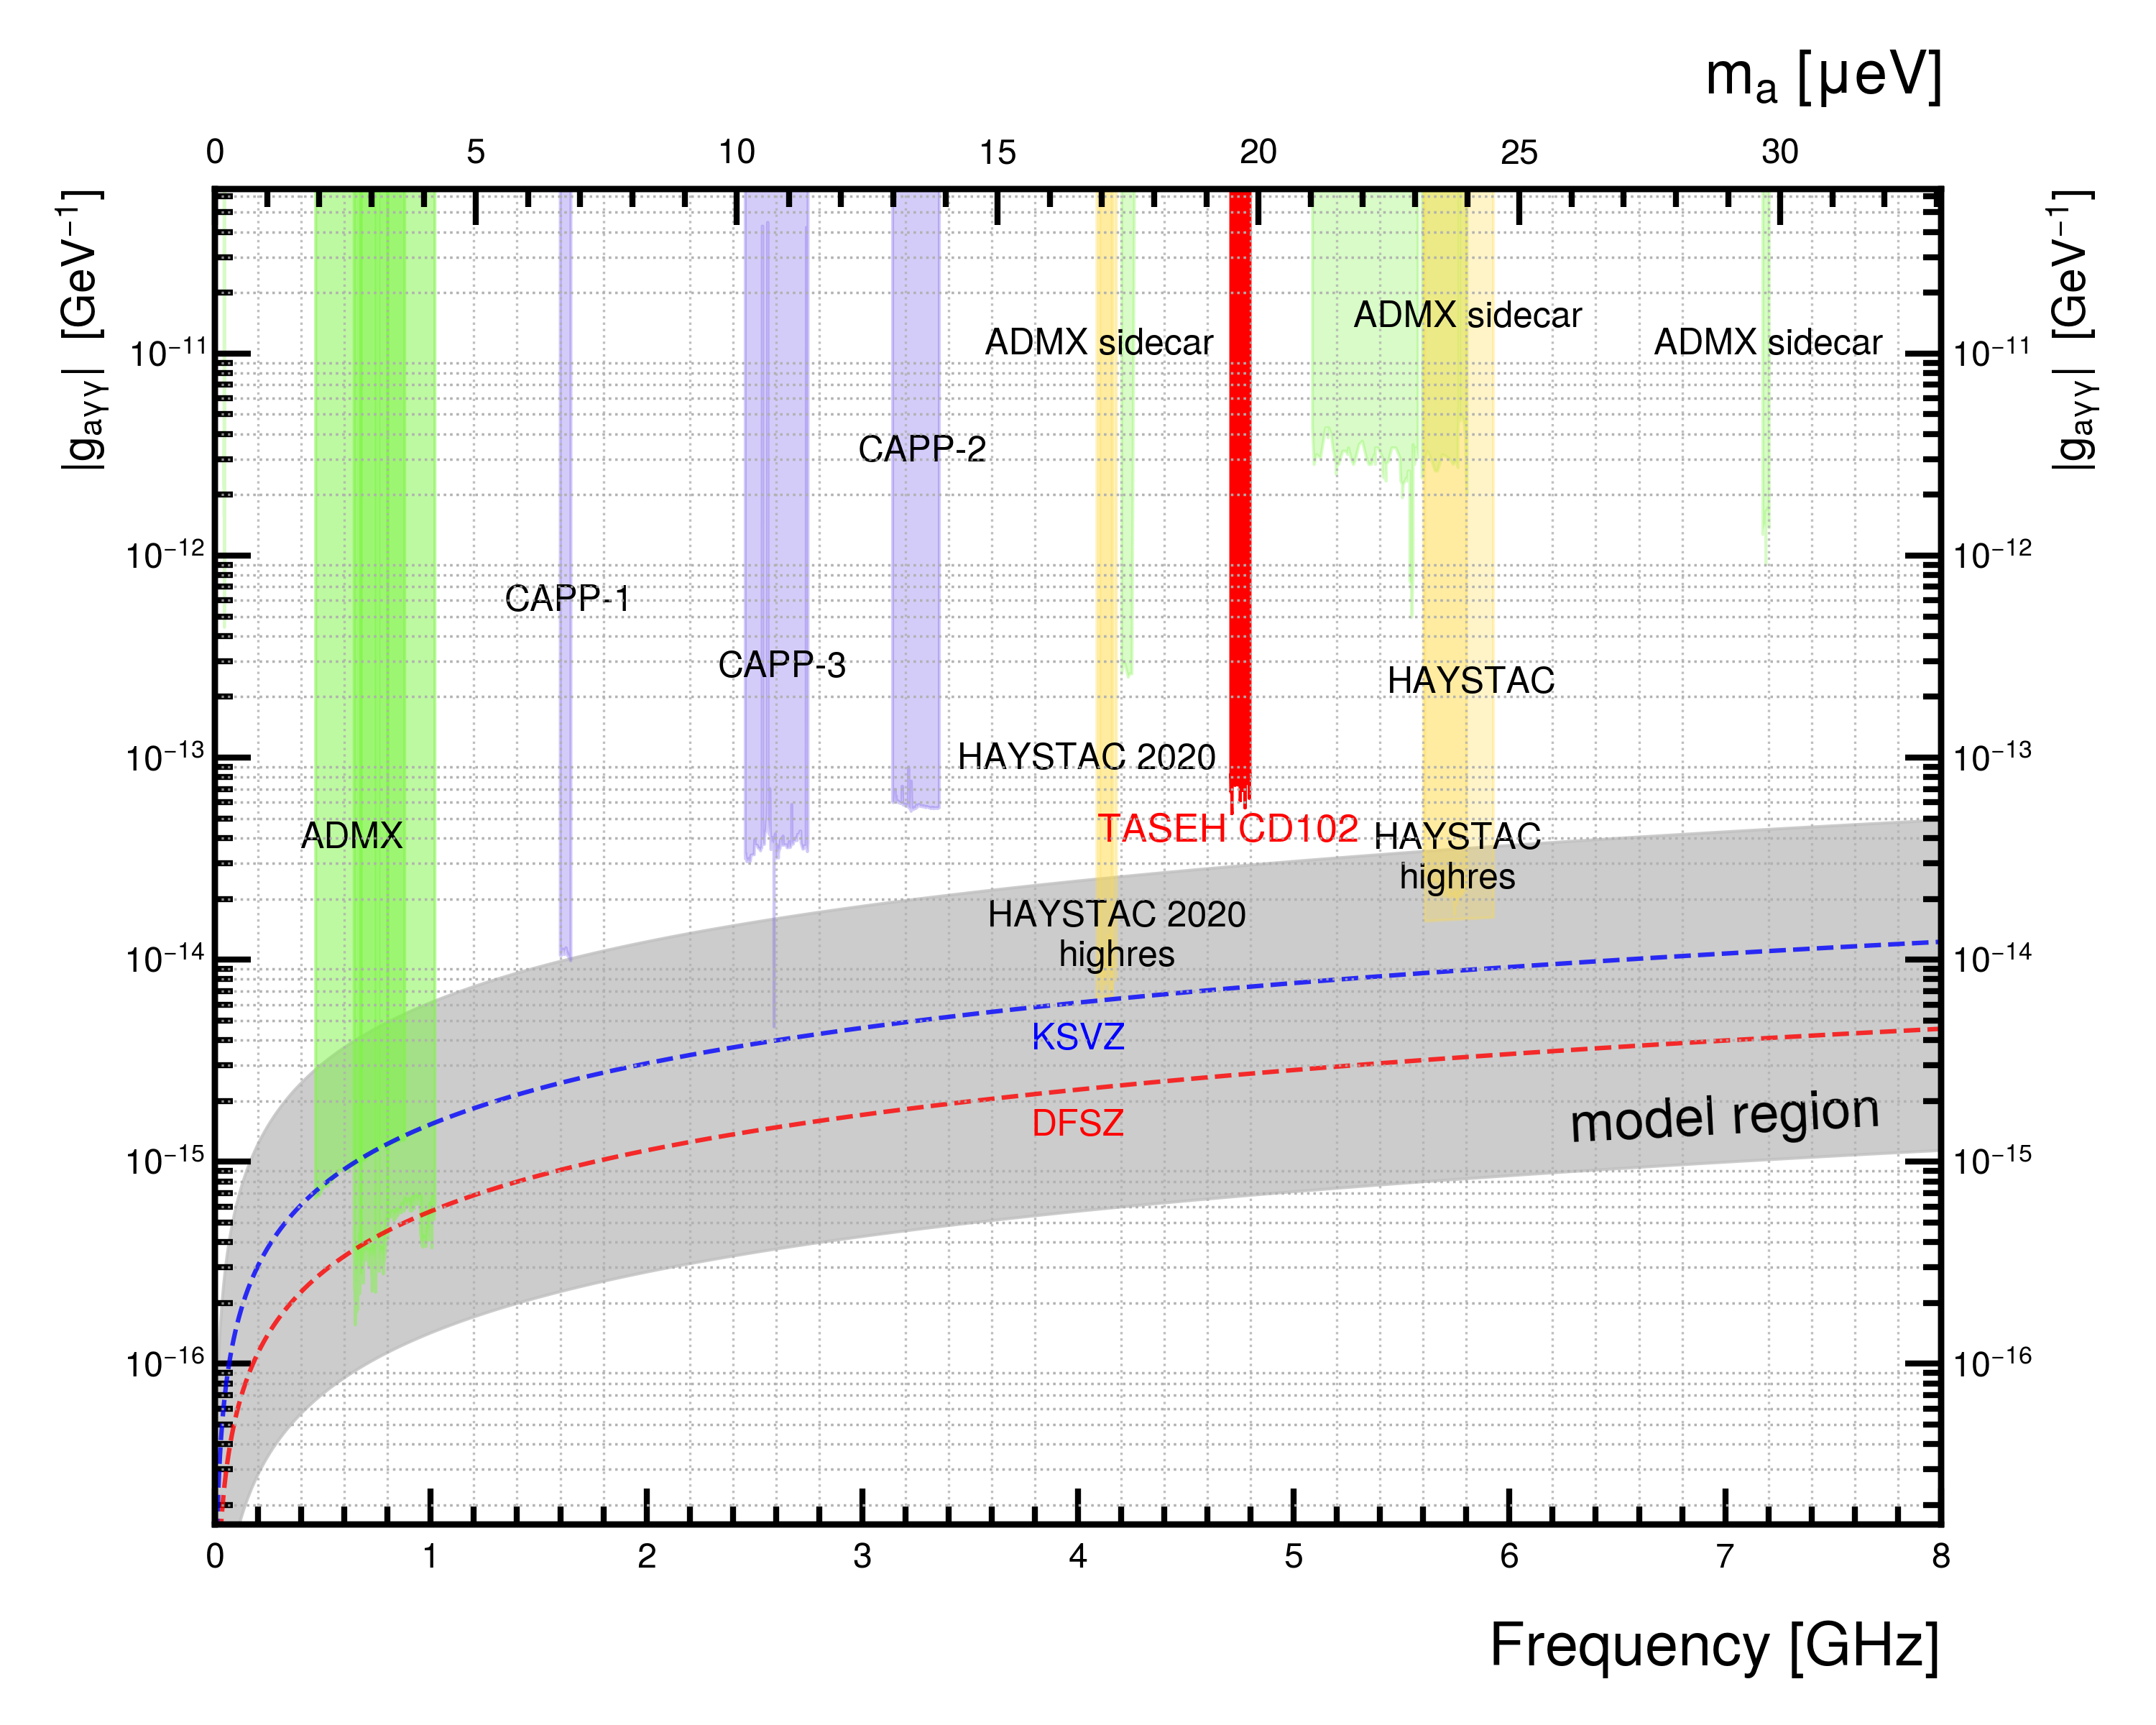
\includegraphics[width=17.2cm]{figures/RealData_limit_allexp.png}
  \caption{The limits on the axion-two-photon coupling \gagg\ for the 
frequency ranges of 0.4--8~GHz, from the CD102 data of TASEH and previous 
searches performed by the ADMX, CAPP, and HAYSTAC Collaborations. The gray 
band indicates the allowed region of \gagg\ vs. $m_a$ from various QCD axion 
models while the blue and red dashed lines are the values predicted by the 
KSVZ and DFSZ benchmark models, respectively.}
  \label{fig:gaggall}
\end{figure*}


\begin{figure} [htbp]
  \centering
 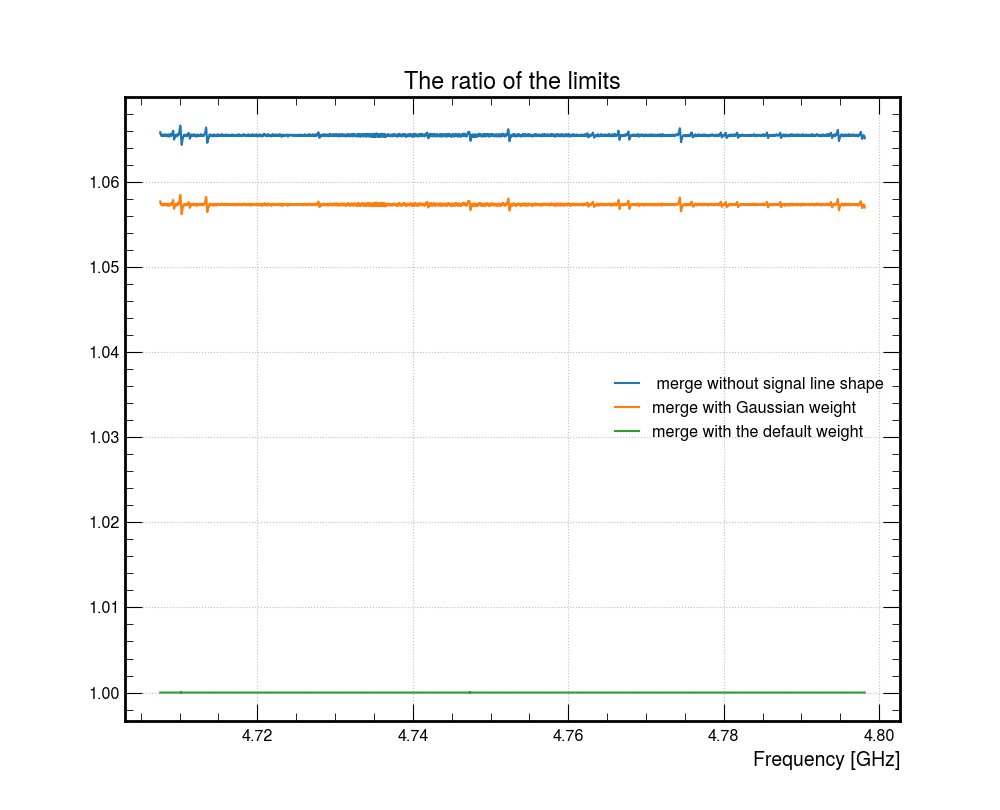
\includegraphics[width=8.6cm]{figures/limitratio_weights.png}
  \caption{The ratios of the limits on \gagg\ from the merging without 
 assuming a signal line shape (blue) and from the merging with a 
 Gaussian weight (orange), with respect to the central 
 results. }
  \label{fig:limitratio}
\end{figure}
